\chapter{Experiments}
\label{ch:experiments}

In this chapter an experiment is presented in order to assert the quality of the proposed planning system. The experiment was designed in manner to present the advantages of the planner, i.e. the importance of the pushing action, for several scenarios. 

\paragraph{First Experiment}
The first experiment presents all the challenges the planners can handle, which are, objects on top of others and objects that need to be moved in order to grasp all of them. 
\begin{figure}[tb]
\centering
\begin{subfigure}[t]{0.45\textwidth}
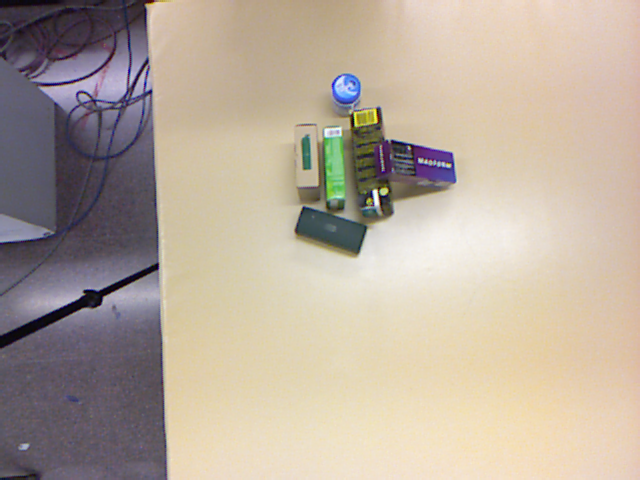
\includegraphics[width=6cm]{Img/experiments/image.png}
\caption{Kinect's view}\label{fig:experiment_good1}
\end{subfigure}
\begin{subfigure}[t]{0.45\textwidth}
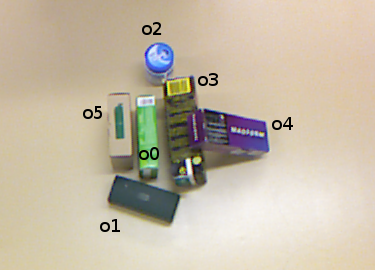
\includegraphics[width=6cm]{Img/experiments/image_labels.png}
\caption{Objects labels.}\label{fig:experiment_good2}
\end{subfigure}
\caption{Kinect's view of the first experiment.}\label{fig:experiment_good}
\end{figure}
In order to get some statistics about the experiment we performed 6 runs. 
We first present the results of a run with some images, and then the actual plan of each run. Finally we discuss the quality of the system in terms of execution and decision time. 

%reference: http://tex.stackexchange.com/questions/53061/insert-image-and-list-inside-a-table
\begin{table}[!h]
\begin{center}
\begin{tabular}{>{\centering\arraybackslash}m{3cm} >{\centering\arraybackslash}m{3cm} >{\centering\arraybackslash}m{3cm} >{\centering\arraybackslash}m{3cm} }
%{>{\centering}m{1in} >{\centering}m{lin} >{\centering}m{lin} >{\centering}m{lin}}
\toprule 
Iteration & Action & Action execution & Result\\
\cmidrule(r){1-1}\cmidrule(lr){2-2}\cmidrule(lr){3-3}\cmidrule(l){4-4}
1 &
\ttt{(push\_dir3 o2)} 
& 
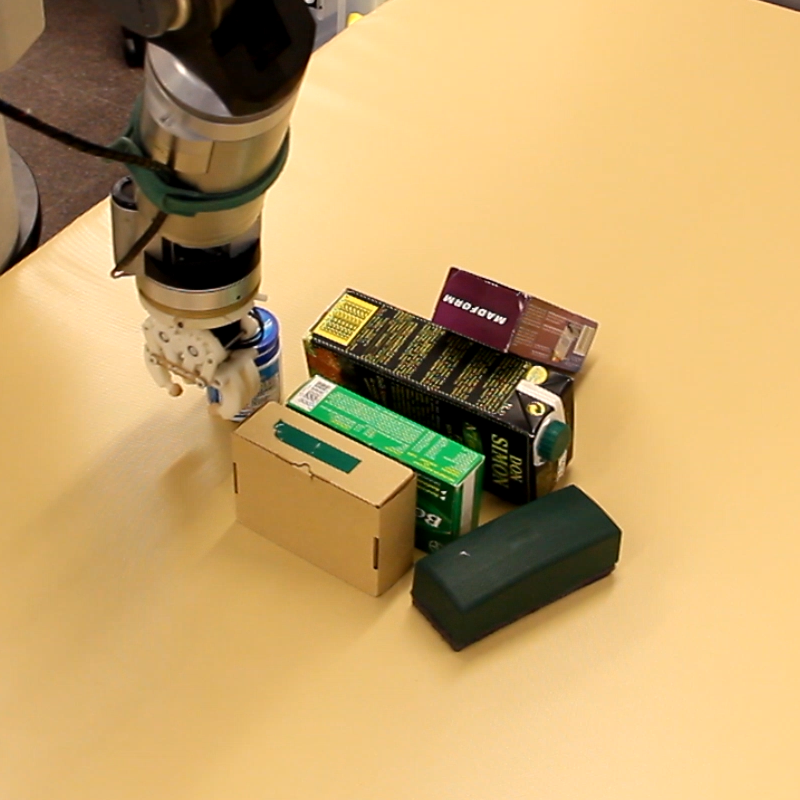
\includegraphics[height=23mm]{Img/experiments/exp_good/action1c.png}
&
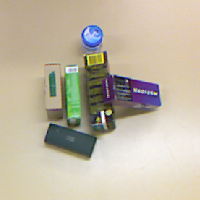
\includegraphics[height=23mm]{Img/experiments/result1.png}
\\
2 &
\ttt{(grasp o2)} 
& 
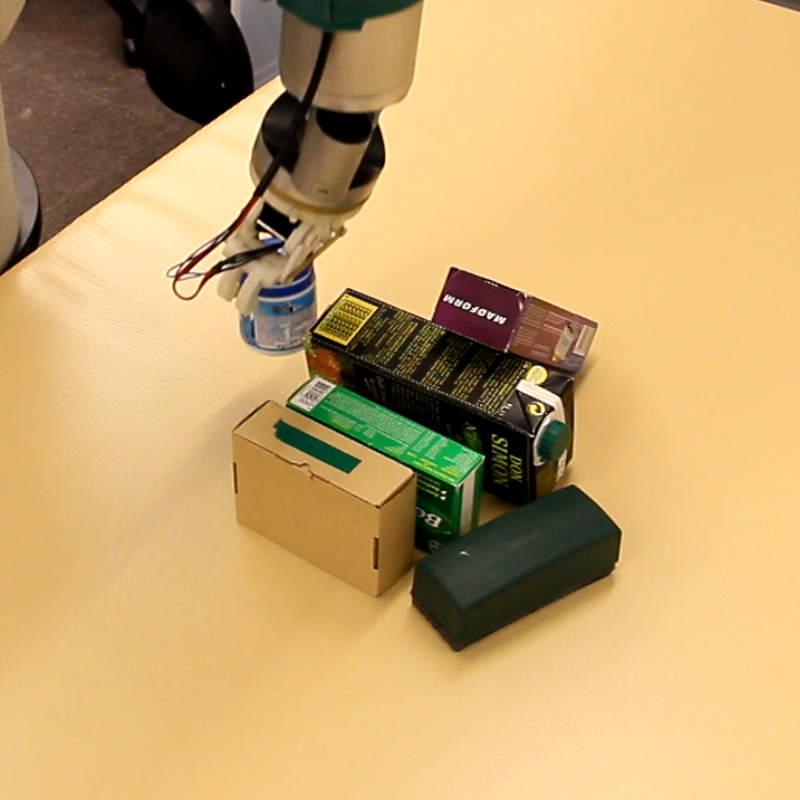
\includegraphics[height=23mm]{Img/experiments/exp_good/action2c.png}
&
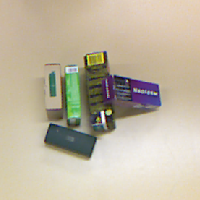
\includegraphics[height=23mm]{Img/experiments/result2.png}
\\
3 &
\ttt{(push\_dir1 o1)} 
& 
%\raisebox{-\totalheight}{
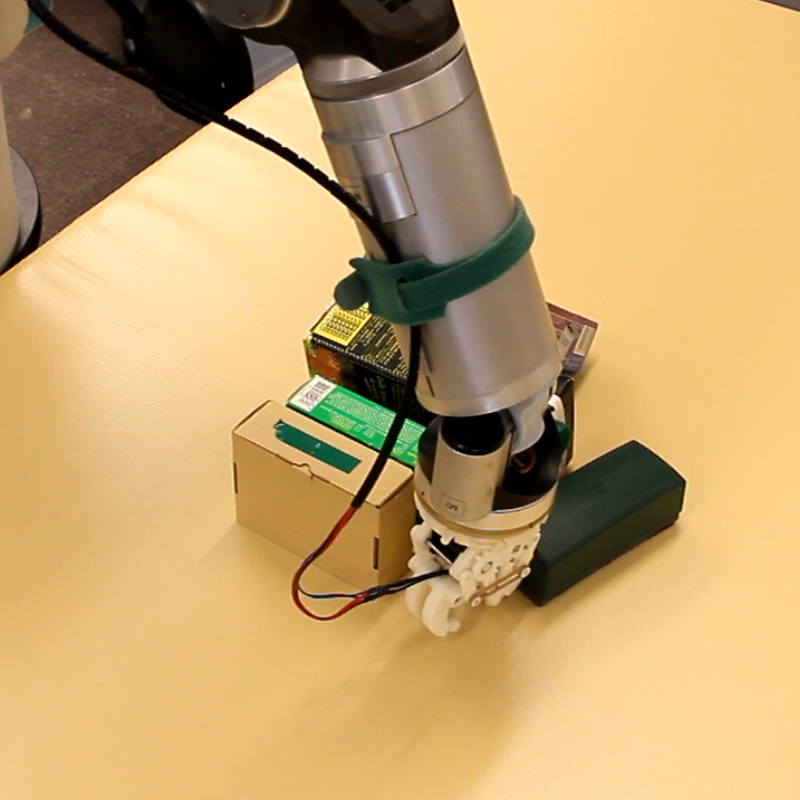
\includegraphics[height=23mm]{Img/experiments/exp_good/action3c.png}%}
&
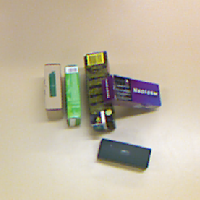
\includegraphics[height=23mm]{Img/experiments/result3.png}
\\
4 &
\ttt{(push\_dir1 o0)} 
& 
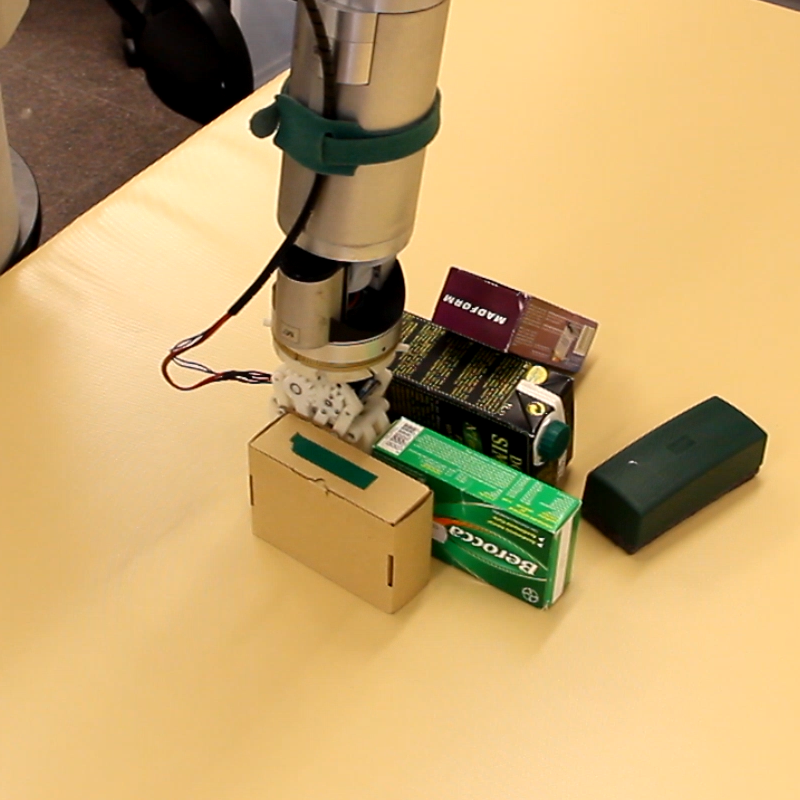
\includegraphics[height=23mm]{Img/experiments/exp_good/action4c.png}
&
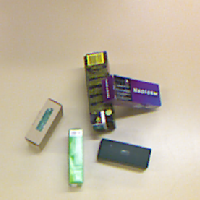
\includegraphics[height=23mm]{Img/experiments/result4.png}
\\
5 &
\ttt{(grasp o4)} 
& 
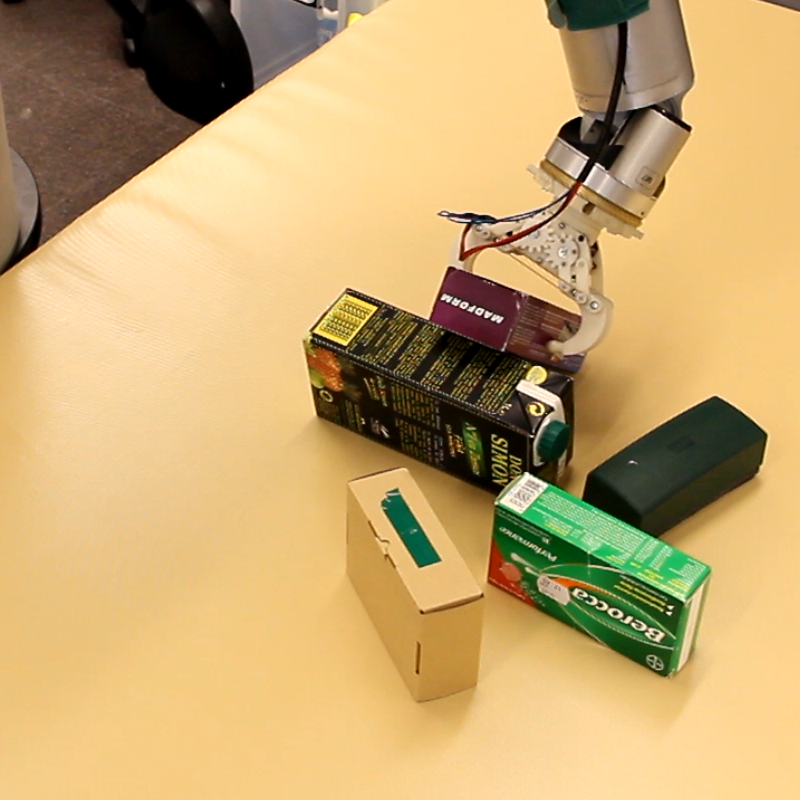
\includegraphics[height=23mm]{Img/experiments/exp_good/action5c.png}
&
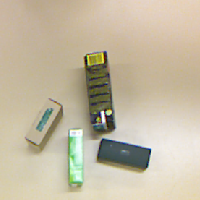
\includegraphics[height=23mm]{Img/experiments/result5.png}
\\
6 &
\ttt{(grasp o1)} 
& 
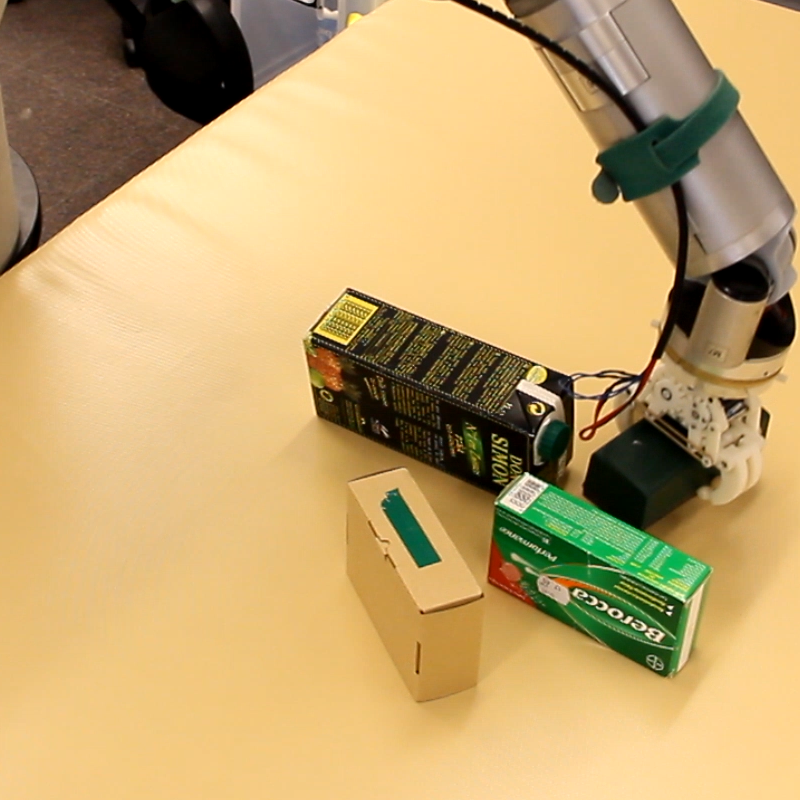
\includegraphics[height=23mm]{Img/experiments/exp_good/action6c.png}
&
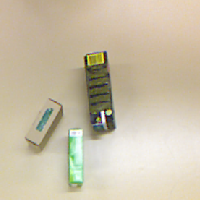
\includegraphics[height=23mm]{Img/experiments/result6.png}
\\
7 &
\ttt{(grasp o3)}
& 
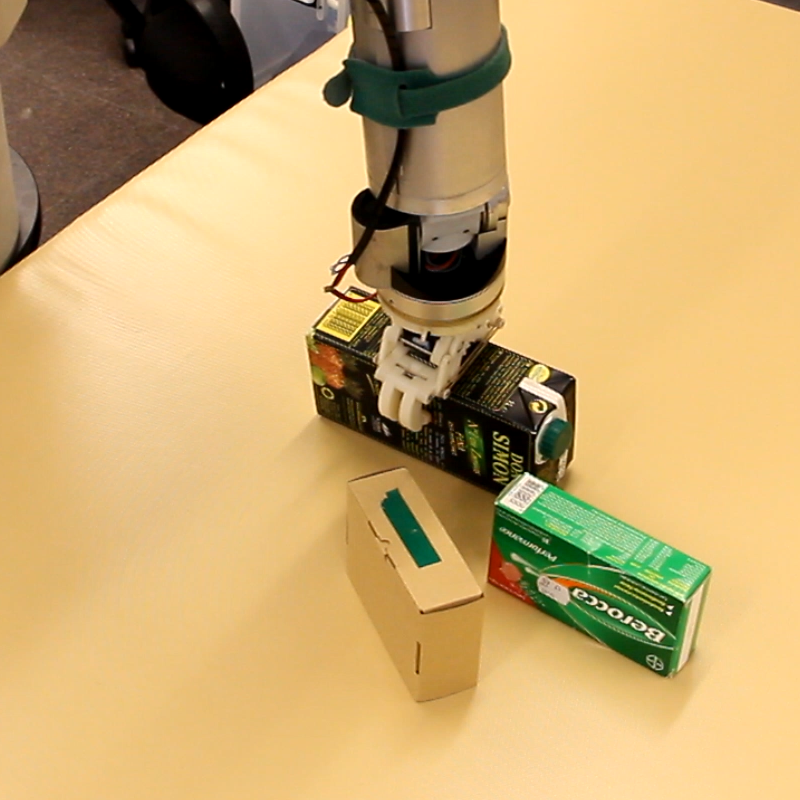
\includegraphics[height=23mm]{Img/experiments/exp_good/action7c.png}
&
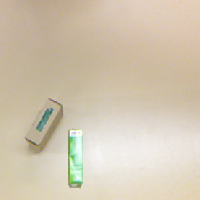
\includegraphics[height=23mm]{Img/experiments/result7.png}
\\
8 &
\ttt{(grasp o0)} 
& 
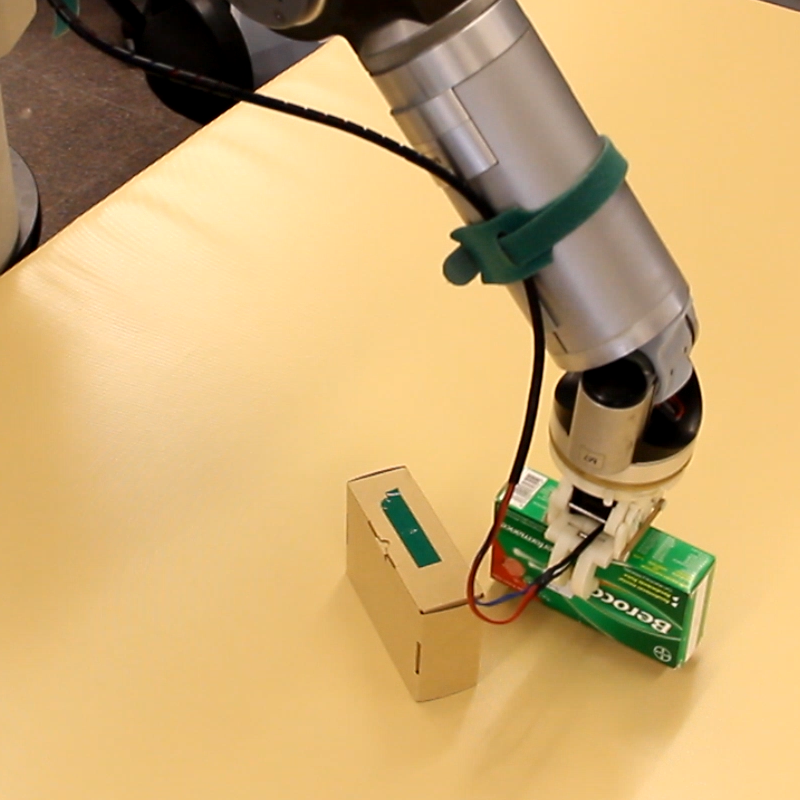
\includegraphics[height=23mm]{Img/experiments/exp_good/action8c.png}
&
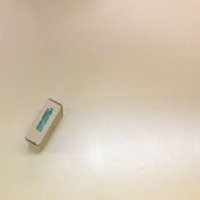
\includegraphics[height=23mm]{Img/experiments/result8.png}
\\
9 &
\ttt{(grasp o5)} 
& 
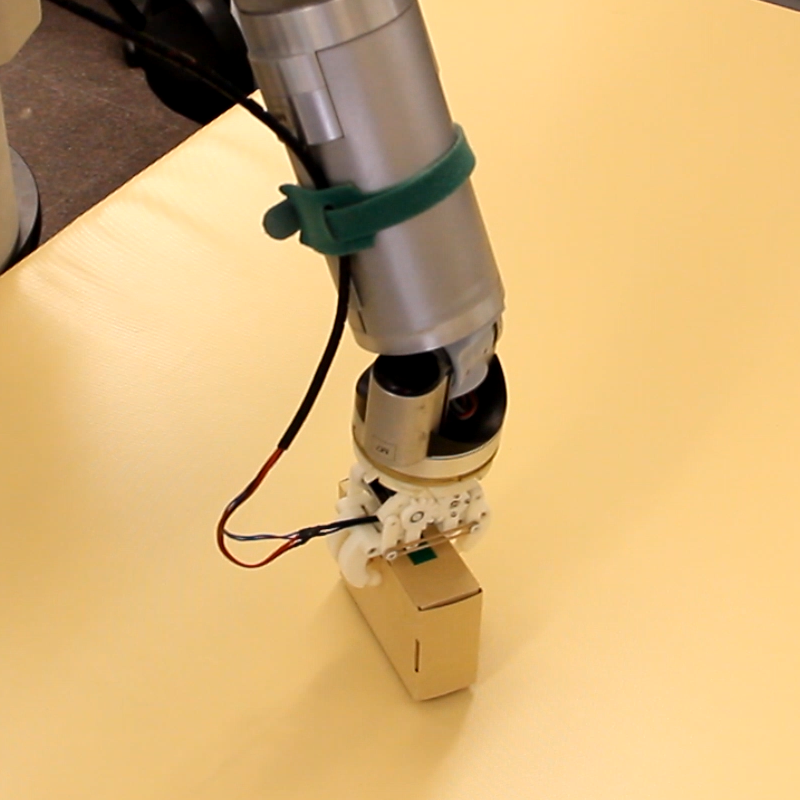
\includegraphics[height=23mm]{Img/experiments/exp_good/action9c.png}
&
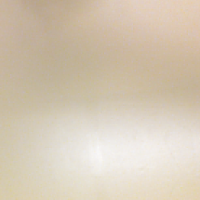
\includegraphics[height=23mm]{Img/experiments/result9.png}
\end{tabular}
\end{center}
\caption{Sequence of action for the experiment of Figure \ref{fig:experiment_good2}}\label{tab:experiment_good}
\end{table}

In Table \ref{tab:experiment_good} the executed plan, for the experiment of Figure \ref{fig:experiment_good} is shown. The plan first decides to push away object \ttt{o2} since it is not able to grasp it due to its grasping pose. In that pose the Kinect is able to see also a side of the object, and therefore its third principal component is such that the grasping pose is the one in the Figure \ref{fig:exp_good_grasp_o2} which is colliding which object \ttt{o3}, therefore it has to move object \ttt{o3} but it cannot because \ttt{o2} hinder that action, another option is pushing away \ttt{o2} and then grasp it. In the next iteration the system takes a new image and now the Kinect is no more able to see one side of \ttt{o2} but only the top surface, so its grasping pose is now a feasible one, and decides to grasp it. Then it push away object \ttt{o1} because it is not possible to grasp it or to move the other objects having \ttt{o1} in such a position. Next it pushes object \ttt{o0}, this action shows the optimality of the planner. If it did not push \ttt{o0} it had to push away first \ttt{o5} and \ttt{o3} to make \ttt{o0} graspable, therefore it saved one action. The outcome of this action is not the expected one since the gripper, during the pushing action, touched slightly \ttt{o5}. In this case is also possible noting the ability of the system to adapt to new situations. Then the robot finishes the task grasping the remaining objects.

\begin{figure}
\centering
\begin{subfigure}[t]{0.45\textwidth}
\centering
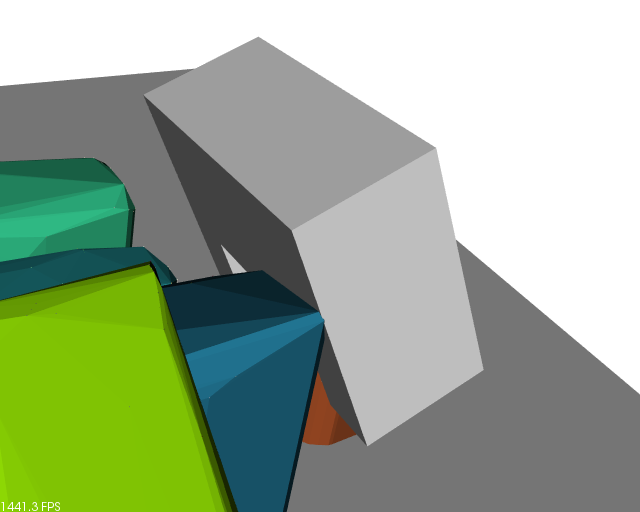
\includegraphics[width = 7cm]{Img/experiments/exp_good/grasp_o2.png}
\caption{}
\end{subfigure}
\begin{subfigure}[t]{0.45\textwidth}
\centering
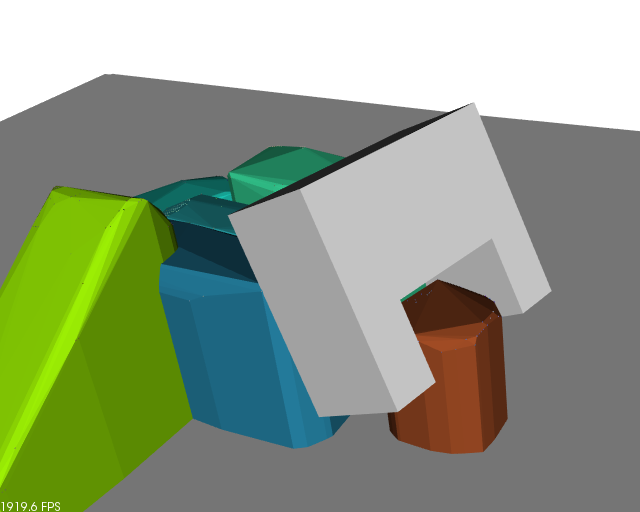
\includegraphics[width = 7cm]{Img/experiments/exp_good/grasp_o2_2.png}
\caption{}
\end{subfigure}
\caption{Collision between the gripper and \ttt{o3} for the grasping pose of object \ttt{o2}.}\label{fig:exp_good_grasp_o2}
\end{figure}

From the experiments done the segmentation has been noted that the segmentation have a strongly importance since, due to the noise of the Kinect, the segmentation was not always the same. Moreover, at the edges the segmentation algorithm had some drawbacks since they tend to be clustered to the bigger adjacent clusters of supervoxels, some edges of an object could be detected as part of the adjacent object. This in several situation can leads to no plan since the object model is not similar to the real object, adn during the computation of collisions the system could detect false collisions. In this case the system can either return that the problem has no solution, so it will take a new images and repeat all the process (in this case the new segmentation could solve the problem), or find anyway a plan.  

In Table ... the executed plans of all the runs for this experiment are reported. The plans differ because of two main reasons: the segmentation is not always the same and in the attempt to reproduce the objects those could have been located not in the exactly poses of previous experiments. 



%%%%%%%%%%% MY COMMENT: The total time here takes into account that the wrong segmentation cases were neglected and also the time needed to save the point clouds
\begin{table}
\caption{Executed plans of the 6 runs for the experiment of Figure \ref{fig:experiment_good}. $N_{actions}$ is the total number of executed actions, $Time_{tot}$ is the total time to solve the task (neglecting the time lost due to the wrong segmentation), $\neg Solution$ is the number of iterations in which no solution was found because of the segmentation and $\neg IK$ is the number of actions that had no solution for the inverse kinematic and the system replaned.}\label{tab:6runs}
\begin{center}
\begin{tabular}{>{\centering\arraybackslash}m{1.5cm} >{\centering\arraybackslash}m{8cm} >{\centering\arraybackslash}m{1.5cm} >{\centering\arraybackslash}m{1.5cm} >{\centering\arraybackslash}m{1.5cm} >{\centering\arraybackslash}m{1cm}}
\toprule 
Run & Plan & $N_{actions}$ & $Time_{tot}$ & $\neg Solution$ & $\neg IK$\\
%\cmidrule(r){1-1}\cmidrule(lr){2-2}\cmidrule(l){3-3}
\toprule
1 & 
\ttt{(push\_dir3 o2)} 
\ttt{(push\_dir1 o1)} 
\ttt{(grasp o1)} 
\ttt{(push\_dir1 o5)} 
\ttt{(grasp o5)} 
\ttt{(push\_dir3 o2)} 
\ttt{(push\_dir1 o0)} 
\ttt{(grasp o0)} 
\ttt{(grasp o3)}
\ttt{(grasp o2)} 
\ttt{(grasp o4)} 
& 11 & $431.5s$ & 3 & 6\\
\toprule
2 &
\ttt{(push\_dir3 o2)} 
\ttt{(grasp o2)} 
\ttt{(push\_dir2 o1)} 
\ttt{(grasp o1)} 
\ttt{(grasp o4)} 
\ttt{(push\_dir2 o0)} 
\ttt{(grasp o0)} 
\ttt{(grasp o3)} 
\ttt{(grasp o5)} 
& 9 & $316.6s$ & 19 & 0\\
\toprule
3 & 
\ttt{(push\_dir3 o2)} 
\ttt{(grasp o2)} 
\ttt{(grasp o4)} 
\ttt{(push\_dir2 o1)} 
\ttt{(grasp o1)} 
\ttt{(push\_dir1 o0)} 
\ttt{(grasp o0)} 
\ttt{(grasp o3)} 
\ttt{(grasp o5)} 
& 9 & $327.6s$ & 3 & 1\\
\toprule
4 & 
\ttt{(grasp o2)} 
\ttt{(grasp o4)} 
\ttt{(push\_dir1 o3)} 
\ttt{(grasp o3)} 
\ttt{(push\_dir1 o1)} 
\ttt{(grasp o1)} 
\ttt{(push\_dir1 o5)} 
\ttt{(grasp o5)} 
\ttt{(grasp o0)} 
& 9 & $294.7s$ & 0 & 0\\
\toprule
5 &
\ttt{(push\_dir3 o2)} 
\ttt{(grasp o4)} 
\ttt{(push\_dir1 o1)} 
\ttt{(grasp o1)} 
\ttt{(push\_dir1 o5)} 
\ttt{(grasp o5)} 
\ttt{(push\_dir1 o0)} 
\ttt{(grasp o0)} 
\ttt{(grasp o3)} 
\ttt{(grasp o2)} 
& 10 & $324.0s$ & 0 & 0\\
\toprule
6 & 
\ttt{(push\_dir3 o2)} 
\ttt{(grasp o2)} 
\ttt{(push\_dir1 o1)} 
\ttt{(push\_dir1 o0)} 
\ttt{(grasp o4)} 
\ttt{(grasp o1)} 
\ttt{(grasp o3)}
\ttt{(grasp o0)} 
\ttt{(grasp o5)} 
& 9 & $298.1s$ & 6 & 0\\
\toprule
\end{tabular}
\end{center}
\end{table}

\paragraph{Comments}
In run 1 the robot grasps object \ttt{o3} although there was \ttt{o4} on top of it. This is because during the execution of \ttt{(push\_dir1 o0)}  action the gripper's cable touch object \ttt{o4} moving it away.  In runs 1,4 and 5 the optimal plan does not return to push object \ttt{o0} as a solution but it returns to push either \ttt{o5} or \ttt{o3}, this also is because of the segmentation. 


For the run 3 the time is high because we filter each point cloud (this slow down the process - fix the code?) - compute the inverse kinematic, when it has no solution its time consuming. 

\begin{figure}[tb]
\centering
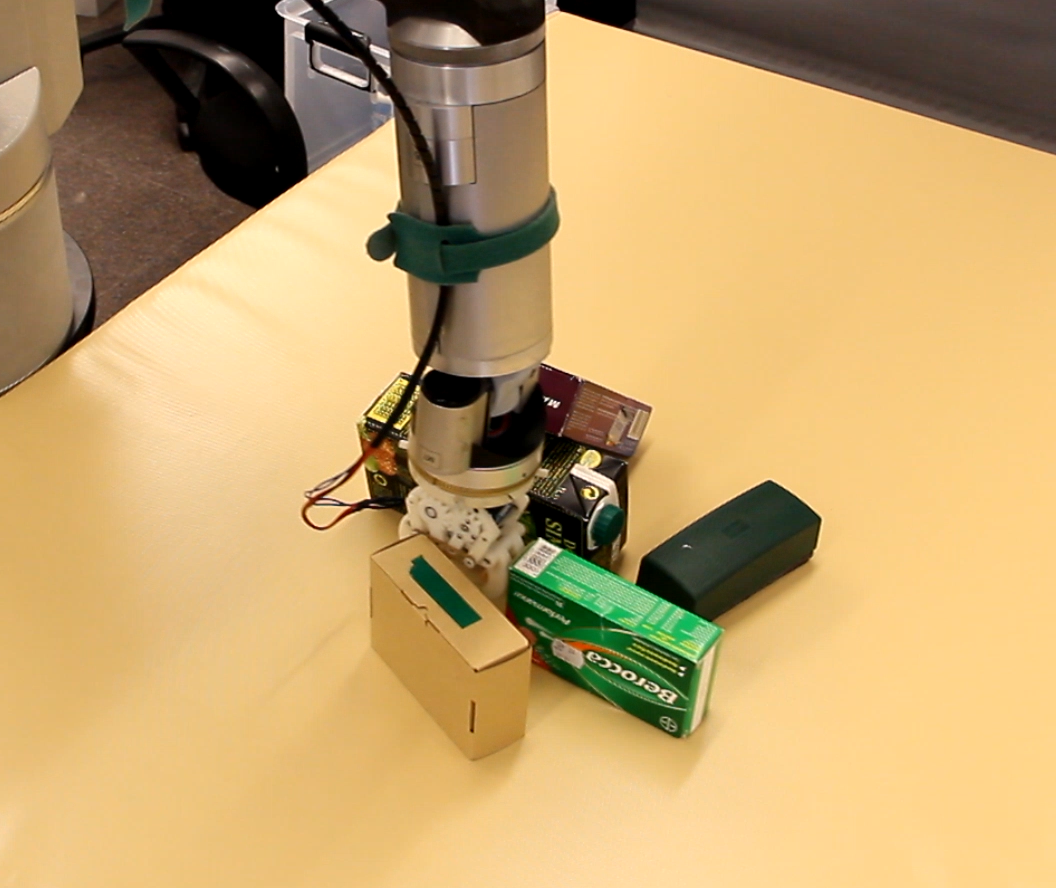
\includegraphics[width=6cm]{Img/experiments/exp_good/pushing_o0c.png}
\caption{Pushing \ttt{o0} the gripper touches also \ttt{o5}.}\label{fig:pushing_o0}
\end{figure}

\begin{figure}[tb]
\centering
\begin{subfigure}[t]{0.45\textwidth}
\centering
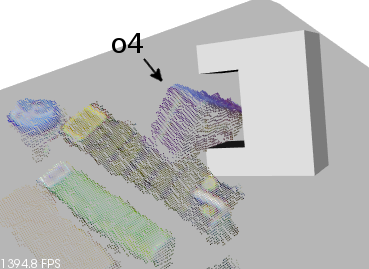
\includegraphics[width=6cm]{Img/experiments/exp_good/grasp_o4.png}
\end{subfigure}
\begin{subfigure}[t]{0.45\textwidth}
\centering
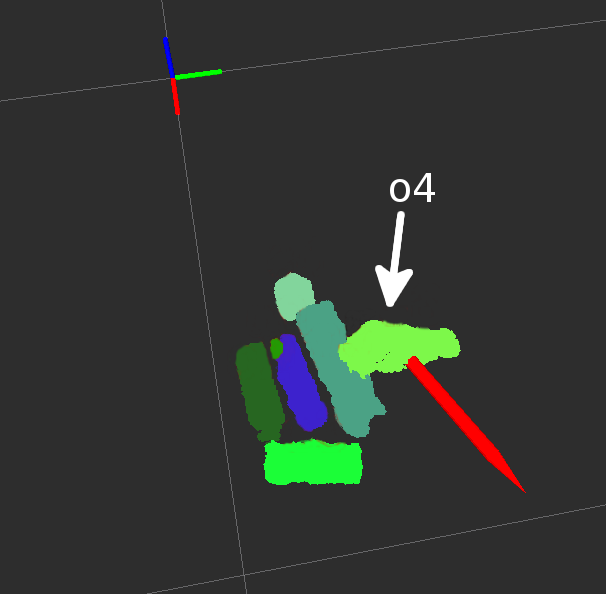
\includegraphics[width=6cm]{Img/experiments/exp_good/grasp_o4_rviz.png}
\end{subfigure}
\caption{Grasping pose of object \ttt{o4} with unfeasible IK.}\label{fig:grasp_o4}
\end{figure}

Due to the strange position of object \ttt{o4} the grasping poses some times were the one depicted in Figure \ref{fig:grasping_pose_o4}. When the planner returned to grasp \ttt{o4} the inverse kinematic returned no solution, so it planed again performing a different action. A feasible grasping pose for object \ttt{o4} was find since, due to the noise of the Kinect, the grasping poses was not always the same and a feasible one could appear. This is because of the height, seen by the Kinect, of \ttt{o4} was higher than its width, so the second principal direction was perpendicular to the top largest surface (Figure \ref{fig:grasp_o4}). 


We will next present some data regarding the times of computing the rpedicates, getting a plan, executing acitons...







\iffalse
In this chapter the performance of the proposed task planner for the considered task is evaluated by performing several experiments with the aim to study the quality, its benefits and its limitations.

To get the quality of the task planner the strategy defined in the article \citep{Benchmarking} by Amignoni et al. In that article they proposed a general method to evaluated the quality of a task planner. 
First they define a functionality benchmark\footnote{A functionality benchmark is a benchmark of specific robotic task. In the case of this thesis a benchmark of the task planner.} thought 4 elements:
\begin{itemize}
\item Description: a high level, general, description of the functionality
\item Input/Output: the information available to the module implementing the function-
ality when executed, and the expected outcome.
\item Benchmarking data: the data needed to perform the evaluation of the performance
of the functional module.
\item Metrics: algorithms to process benchmarking data in an objective way.
\end{itemize}

Regarding the benchmarking of a task planner those elements are defined as:
\begin{itemize}
\item [\textbf{Description:}] Given a initial state and a goal state find a set of actions to reach the goal.
\item [\textbf{Input/Output:}] The inputs are the PDDL domain and problem descriptions. The output is a plan expressed as sequence of actions.
\item [\textbf{Benchmarking data:}] Some data has to be supplied by the robot, including: the input
given to the planner, the output (i.e., the plan) delivered by the planner, and the
performance data for the planner (e.g., memory and time needed). According to
the planning approach, other data might be required. Other data will be possibly collected when a plan is
actually executed, including: time needed to execute each action and time needed
to execute the whole plan.
\item [\textbf{Metrics:}] Metrics are mainly related to good plan quality and to solving time. The target of benchmarking task planning is twofold: to asses the quality of the
plan produced (e.g., in terms of the cost for executing it and its likelihood to succeed) and to assess the quality of the
planning process (i.e., how fast is the plan generated and how much resources are needed to do so). Possible metrics are:
\begin{itemize}
\item \textsl{Levenshtein distance}\footnote{\href{https://en.wikipedia.org/wiki/Levenshtein_distance} {https://en.wikipedia.org/wiki/Levenshtein\_distance}} is a metric that specifies the distance between two strings, in this case a plan can be though as a sequence of character, where each action with a determined object of interest is a character of the string. The Levenshtein distance between the two lists is calculated to measure the quality of the plan. Levenshtein distance
$L_{A,B}(|A|,|B|)$ between two lists A and B is calculated as
\begin{align*}
L_{A,B}(i,j) &= \max(i,j) \qquad if \quad \min(i,j)=0 \\
L_{A,B}(i,j) &= \min(L_{A,B}(i-1,j)+1, \\
& \qquad \quad L_{A,B}(i,j-1)+1,
\\ & \qquad \quad L_{A,B}(i-1,j-1)+1_{a_i \neq b_i})
\qquad otherwise
\end{align*}
where $|A|$ is the length of plan A, and $1_{a_i \neq b_i}$ is equal to 0 if the action $a_i$ is the same of action $b_i$. This metric will be used to evaluate the distance between the optimal plan returned by the planner in the first frame and the real executed plan. 
\item Number of actions correctly performed in the correct order (e.g., number of
objects delivered to their correct destination). 
\item Time required to construct a plan and time to perform it. 
\end{itemize}
\end{itemize}
We will also evaluate the difference of executing the initial plan and executing the plan with the replanning technique in terms of time and number of correct actions. As well also the number of bad, or dangerous, object manipulations due to the lack of replanning, lack of probability and geometric constraints in the planner . 

It is important highlighting that what has been done is not a benchmarking since no comparison is done with other state of the art planners, but the commented guideline for benchmarks has been used in order to get some useful metrics in order to assert the quality of the planner. 

Kinds of possible experiment to do:
\begin{itemize}
\item show experiments first trying only separating the object (infinite loop behaviour) and then coupling the grasping action. 
\item Show the results of the planner with the pushing length chosen not accordingly to the surrounding objects but accordingly to the pushed one. From that comment the improvements.
\item Show normal experiment where everything works
\item Show situation why we are going to consider the risk as cost in the action. 
\end{itemize}

Metrics to considers:
\begin{itemize}
\item number of objects
\item segmentation time
\item Total solution time
\item planning time
\item total solution
\item Inverse kinematics solution time (this will probably used to justify the backtracking method)
\item Predicates time computation (maybe add collision checking time in )
\end{itemize}


Find a way to get the computational complexity. 

\begin{figure}
\centering
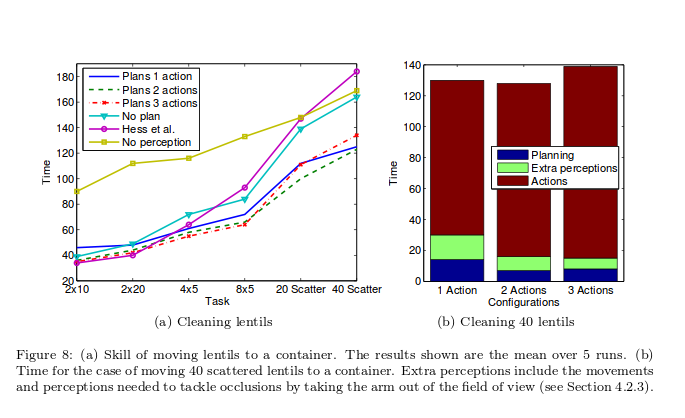
\includegraphics[width=\textwidth]{Img/general/experiments.png}
\end{figure}

\begin{itemize}
\item 2 experiments in which everything works
\item experiment which shows the limitaiton of the planner
\end{itemize}

\fi